
%%%%%%%%%%%%%%%%%%%%%%% file typeinst.tex %%%%%%%%%%%%%%%%%%%%%%%%%
%
% This is the LaTeX source for the instructions to authors using
% the LaTeX document class 'llncs.cls' for contributions to
% the Lecture Notes in Computer Sciences series.
% http://www.springer.com/lncs       Springer Heidelberg 2006/05/04
%
% It may be used as a template for your own input - copy it
% to a new file with a new name and use it as the basis
% for your article.
%
% NB: the document class 'llncs' has its own and detailed documentation, see
% ftp://ftp.springer.de/data/pubftp/pub/tex/latex/llncs/latex2e/llncsdoc.pdf
%
%%%%%%%%%%%%%%%%%%%%%%%%%%%%%%%%%%%%%%%%%%%%%%%%%%%%%%%%%%%%%%%%%%%


\documentclass[runningheads,a4paper]{llncs}

\usepackage{amssymb}
\setcounter{tocdepth}{3}
\usepackage{graphicx}

\usepackage{url}

\selectlanguage{slovene}
\usepackage [slovene]{babel}
\usepackage[hidelinks]{hyperref}

\urldef{\mailsa}\path|{matej.hrlec.fri, gal.kos.fri}@gmail.com|    
\newcommand{\keywords}[1]{\par\addvspace\baselineskip
\noindent\keywordname\enspace\ignorespaces#1}

% CUSTOM IMPORTS
% fixed image postion
\usepackage{float}
\usepackage[export]{adjustbox}

\begin{document}

\mainmatter  % start of an individual contribution

% first the title is needed
\title{Interaktivni projekt s pomočjo uporabe CNN}

% a short form should be given in case it is too long for the running head
\titlerunning{Interaktivni projekt s pomočjo uporabo CNN}

% the name(s) of the author(s) follow(s) next
%
% NB: Chinese authors should write their first names(s) in front of
% their surnames. This ensures that the names appear correctly in
% the running heads and the author index.
%
\author{Matej Hrlec, Gal Kos}
%
% (feature abused for this document to repeat the title also on left hand pages)

% the affiliations are given next; don't give your e-mail address
% unless you accept that it will be published
\institute{Fakulteta za računalništvo in informatiko,\\
Večna pot 113, 1000 Ljubljana\\}

%
% NB: a more complex sample for affiliations and the mapping to the
% corresponding authors can be found in the file "llncs.dem"
% (search for the string "\mainmatter" where a contribution starts).
% "llncs.dem" accompanies the document class "llncs.cls".
%

\toctitle{CNN}
\tocauthor{Authors' Instructions}
\maketitle


\begin{abstract}
Ker obstaja precej knjižnic, ki uporabljajo konvolucijske nevronske mreže za obdelavo podatkov, smo v okviru tega projekta opravili pregled te panoge strojnega učenja ter implementirali sistem za zaznavo in obdelavo slik s pomočjo knjižnic CNN. Razvili smo klasificiranje objektov v slikah in stiliranje zaznanih regij s prenosom sloga umetniških slik.
%\keywords{We would like to encourage you to list your keywords within
%the abstract section}
\end{abstract}


\section{Uvod}
V zadnjih letih se je začel nagel razvoj sistemov strojnega učenja, ki temeljijo na simuliranju človeškega razmišljanja. To je v veliki možno zaradi velikega napredka na področju programerskih vmesnikih za izvajanje masovno paralelizirane kode na grafičnih karticah. Poleg tega so se kapacitete grafičnih pomnilnikov in pomnilniških povezav precej povečale, kar omogoča obdelavo velikih podatkovnih baz.

V okviru tega projekta smo se osredotočili predvsem na uporabo konvolucijskih nevronskih mrež, bolj natančno na njihovo uporabo pri obdelavi in klasifikaciji slik. Z uporabo in povezovanjem knjižnic, ki podpirajo določene operacije nad slikami, smo implementirali sistem, ki predstavlja praktično uporabo zgornjih funkcionalnosti.

\raggedbottom
\section{Opis tematike in pregled področja}

\subsection{Nevronske mreže}
Umetne nevronske mreže (angl. \textit{Artificial neural networks} - ANNs) so računski model, ki temelji na veliki zbirki povezav preprostih nevronskih enot oziroma nevronov (angl. \textit{artificial neurons}), ki so po obnašanju sorodni možganskim aksonom\cite{wiki:ANN}. 

Vsaka nevronska enota je povezana z mnogimi drugimi, povezave lahko povečajo ali zavirajo stanje aktiviranja sosednjih nevronskih enot. Posamezna nevronska enota izračunava izhode s pomočjo funkcije seštevanja. Pogosto obstaja tudi pragovna funkcija (angl. \textit{threshold function}) na vsaki povezavi ali na enoti sami, ki določa stopnjo, ki jo mora signal preseči preden se lahko razširi do sosednjih nevronov. Nevronski sistemi se odločanja naučijo samostojno, tako da niso eksplicitno programirani in se odlikujejo predvsem na področjih, kjer je rešitev ali zaznavanje značilnosti težko izraziti v tradicionalnem računalniškem programu.

Nevronske mreže so običajno sestavljene iz več plasti, pri čemer se signalna pot razteza od prve (vhodne) do zadnje (izhodne) plasti nevronskih enot kot je vidno na sliki \ref{fig:layersANN}. Sodobna nevronska omrežja so v smislu simulacije pretočnejša, zato pri tovrstnih omrežjih povezave interaktirajo veliko bolj kaotično in kompleksno. Najnaprednejše so dinamične nevronske mreže, ki lahko na podlagi pravil tvorijo nove povezave in celo ustvarjajo nove nevronske enote ali jih onemogočajo.

\begin{figure}[H]
\centering
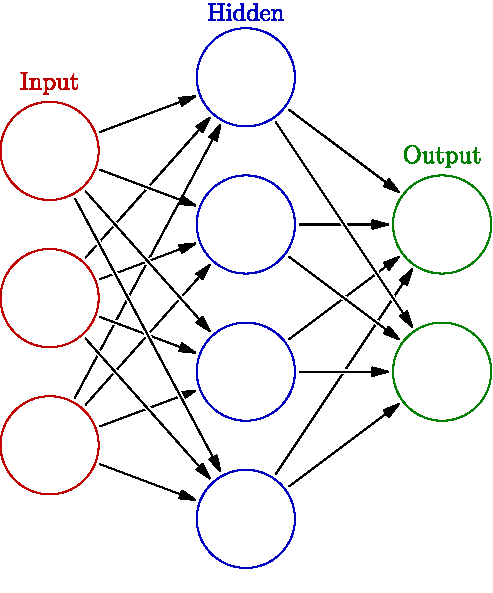
\includegraphics[width=55mm]{figures/Colored_neural_network.pdf}
% ref: https://en.wikipedia.org/wiki/Artificial_neural_network#/media/File:Colored_neural_network.svg
\caption{Vhodna, skrita in izhodna plast pri umetnih nevronskih mrežah}
\label{fig:layersANN}
\end{figure}

Cilj nevronskih mrež je reševanje problemov na enak način, kot bi jih reševali človeški možgani, čeprav so veliko bolj abstraktne. Sodobni projekti uporabljajo nevronske mreže, ki so običajno sestavljene iz nekaj tisoč do nekaj milijonov povezav, kar je še vedno velikokrat manj kompleksno od človeških možganov in so bolj podobne računski moči črva.

Zanimiv vidik nevronskih sistemov je, da so nepredvidljivi glede tega, kako uspešni bodo pri samostojnem učenju. Po tem, ko se naučijo na učnih podatkih, nekateri dobro rešujejo probleme, medtem ko drugi pri reševanju novih problemov niso tako uspešni. Proces učenja običajno zahteva več tisoč ciklov interakcije. Podobno kot pri ostalih metodah strojnega učenja, torej sistemih, ki se učijo iz podatkov, se tudi nevronske mreže uporabljajo za reševanje širokega spektra različnih nalog. Dober primer sta računalniški vid in prepoznavanje govora, ki sta težko rešljiva problema z uporabo tradicionalnega programiranja.

\subsection{Konvolucijske nevronske mreže}

Konvolucijske nevronske mreže (angl. \textit{convolutional neural network} - CNN) so vrsta umetnih nevronskih mrež, pri katerih se vzorec povezljivosti med nevronskimi enotami zgleduje po ureditvi vidnega korteksa pri živalih\cite{wiki:CNN}. Posamezni kortikalni nevroni se odzivajo na dražljaje v omejeni prostorski regiji oziroma receptivnem polju. Tovrstna polja različnih nevronov se delno prekrivajo, tako da vidno polje razdelijo na ploščice. Odziv posameznega nevrona na dražljaje v svojem receptivnem polju lahko matematično aproksimiramo z operacijo konvolucije. Konvolucijska omrežja izhajajo iz bioloških procesov in so variacije večplastnih zaznav, ki katerih je predprocesiranje minimalno. Konvolucijske nevronske mreže se uporabljajo v aplikacijah za prepoznavo slik in videa, v priporočilnih sistemih in pri obdelavi naravnega jezika.

Konvolucijske nevronske mreže so torej različice večslojnih zaznavanj (angl. \textit{multilayer perceptron} - MLP), ki so osnovane tako, da lahko posnemajo vidni korteks. Mreže CNN imajo naslednje značilne lastnosti:
\begin{itemize}
\item \textbf{3D volumni nevronov:} Sloji CNN imajo nevrone razporejene v treh dimenzijah: širina, dolžina in globina, kot je vidno na sliki \ref{fig:layersCNN}. Nevroni znotraj sloja so povezani samo z majhnim območjem plasti pred njih - receptivnim poljem. Različni tipi plasti, tako lokalno kot globalno povezani, so nakopičeni, s čimer tvorijo arhitekturo CNN.

\item \textbf{Lokalna povezljivost:} V skladu s konceptom receptivnih polj mreže CNN izkoriščajo prostorsko-lokalno korelacijo z uveljavljanjem lokalne povezljivosti med nevroni sosednjih plasti. Arhitektura tako zagotavlja, da naučeni filtri ustvarijo najmočnejši odziv na prostorsko-lokalni vhodni vzorec. Kopičenje več takih plasti vodi do nelinearnih filtrov, ki postajajo vedno bolj globalni, torej se odzivajo na vedno večje območje. To omogoča omrežju, da najprej ustvari dobre predstavitve manjših delov vhoda in nato te majhne dele združi v predstavitve večjih področij.

\item \textbf{Deljene uteži:} Pri mrežah CNN je vsak filter repliciran v celotnem vidnem polju. Te replicirane enote si delijo enako parametrizacijo, torej vektor uteži in začetno vrednost, s čimer tvorijo mapo značilk. Tako vsi nevroni v dani konvolucijski plasti zaznavajo povsem enako funkcijo. Takšno podvajanje nevronskih enot omogoča, da so lastnosti detektirane ne glede na njihov položaj v vidnem polju, kar predstavlja translacijsko invarianco.
\end{itemize}

\begin{figure}[H]
\centering
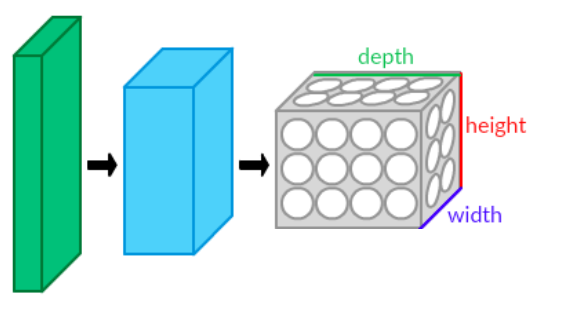
\includegraphics[width=80mm]{figures/Conv_layers.png}
% ref: https://en.wikipedia.org/wiki/Convolutional_neural_network#/media/File:Conv_layers.png
\caption{Plasti CNN so razporejene v treh dimenzijah (širina, dolžina in globina)}
\label{fig:layersCNN}
\end{figure}

Skupaj zgornje lastnosti omogočajo mrežam CNN doseganje boljše generalizacije problemov. Delitev uteži dramatično zmanjša število prosti parametrov, ki se jih je potrebno naučiti, s čimer znižuje pomnilniške zahteve za delovanje mreže. Zmanjšanje zahtev po virih omogoča učenje večjih in močnejših nevronskih omrežij. Na sliki \ref{fig:archCNN} referenco je vidna tipična arhitektura CNN.

\begin{figure}[H]
\centering
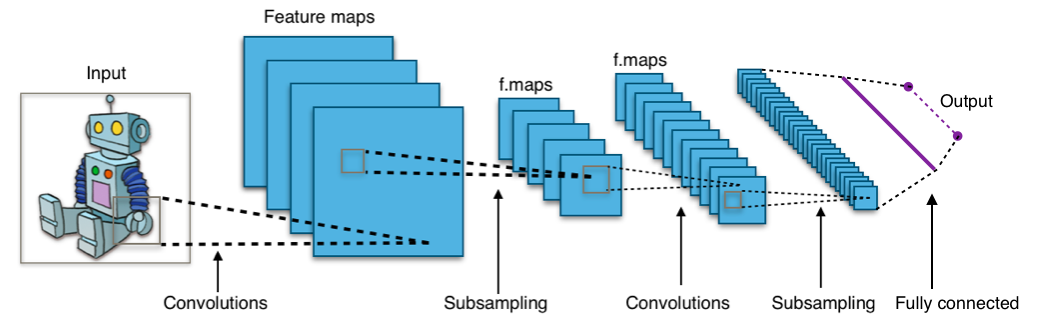
\includegraphics[width=120mm]{figures/Typical_cnn.png}
% ref: https://en.wikipedia.org/wiki/Convolutional_neural_network#/media/File:Typical_cnn.png
\caption{Tipična arhitektura konvolucijskih nevronskih mrež}
\label{fig:archCNN}
\end{figure}

\subsection{Projekt Darknet}
Darknet je odprtokodno ogrodje (angl. \textit{framework}) za delo z nevronskimi mrežami sprogramirano v jeziku C in platformi CUDA (angl. \textit{Compute Unified Device Architecture})\cite{darknet13}. Ogrodje podpira procesorsko in grafično podprto računanje.

Darknet – YOLO (angl. \textit{you only look once}) je realnočasovni sistem za zaznavanje objektov na slikah s pomočjo mrež CNN, ki lahko zazna preko 9000 kategorij objektov. 

Sistem uporablja enotno nevronsko omrežje na celotni sliki, s čimer razdeli sliko na regije, napove omejitvena polja in verjetnosti za vsako regijo. Omejitvena polja so utežena z napovedano verjetnostjo. Sistem detektira celotno sliko v času testiranja, zato so napovedi izračunane glede na globalni kontekst slike. Sistem natisne objekte, ki jih je zaznal in izračuna zaupanje (angl. \textit{confidence}) in kako dolgo je trajalo da je objekta našel. V okviru projekta je na voljo več pred-naučenih modelov.  Primer detekcije je viden na sliki \ref{fig:darknetExample}.

\begin{figure}[H]
\centering
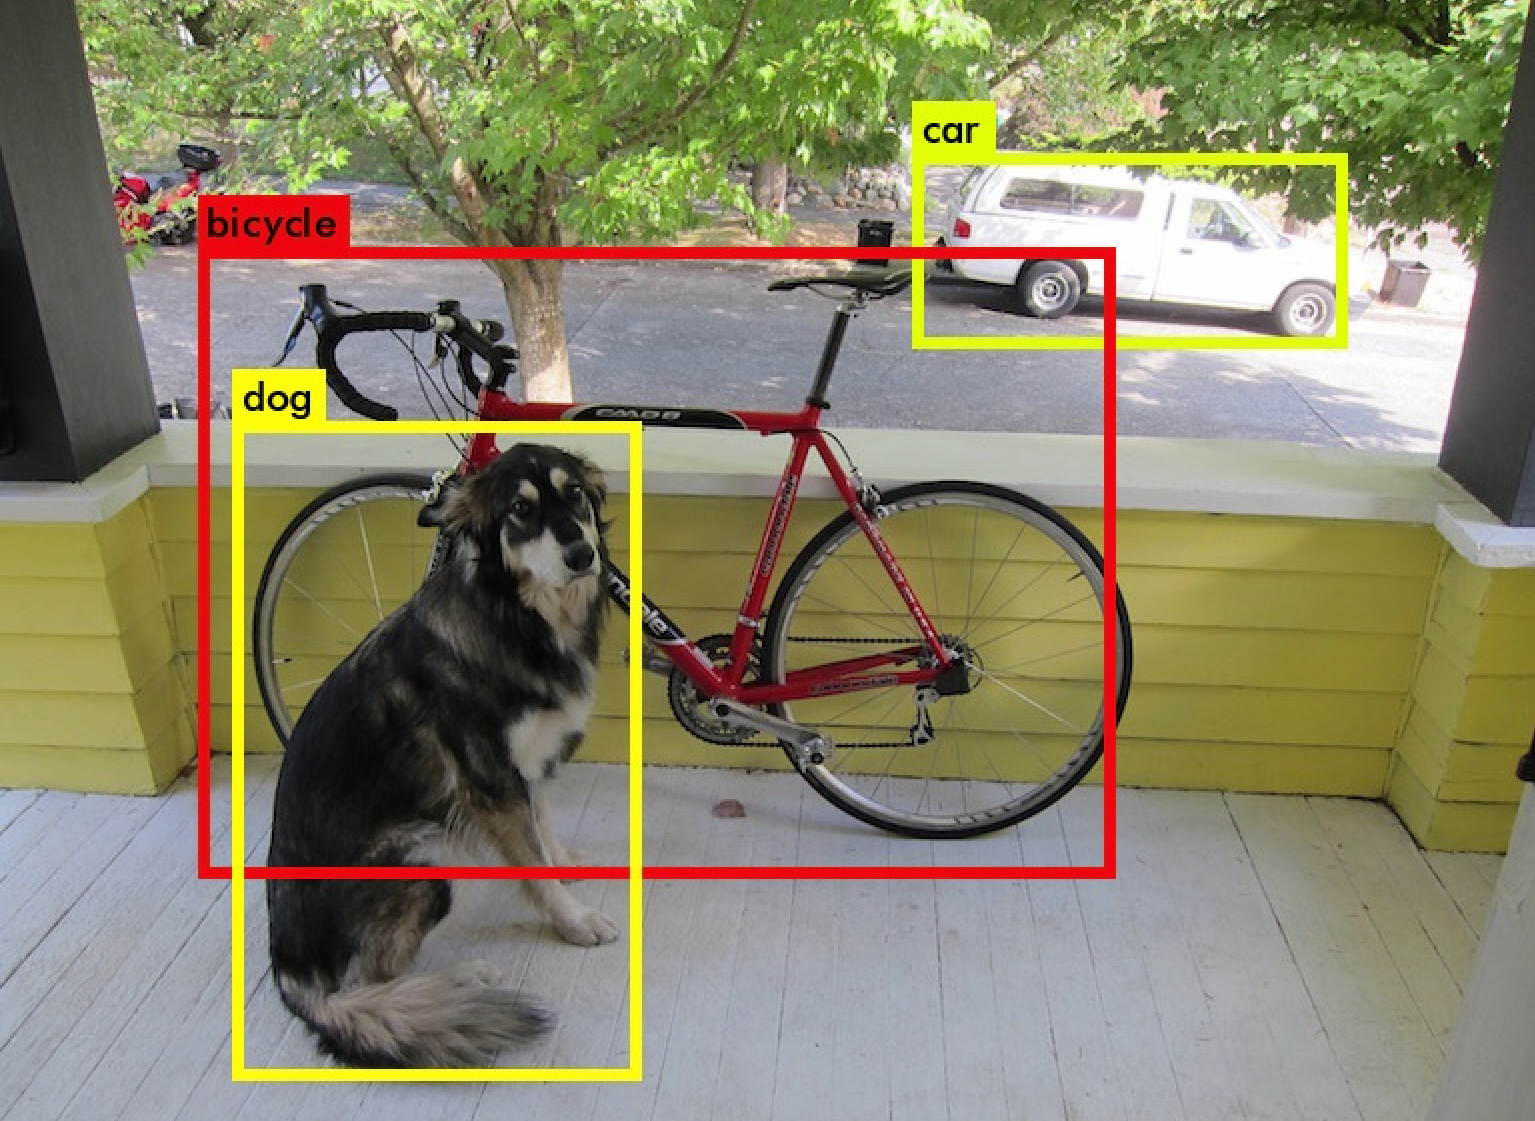
\includegraphics[width=90mm]{figures/darknetExample.png}
% https://pjreddie.com/media/image/Screen_Shot_2016-11-17_at_11.14.54_AM.png
\caption{Primer detekcije z uporabo sistema Darknet - YOLO}
\label{fig:darknetExample}
\end{figure}

\subsection{TensorFlow}
S pomočjo uporabe odprtokodne programske knjižnice lahko razvijamo sisteme, ki so sposobni grajenja in učenja nevronskih mrež. S tem lahko zaznavamo vzorce in povezave podobno kot smo to sposobni ljudje.

Arhitektura API-ja omogoča uporabo CPE (centralna procesna enota) ali GPE (grafična procesna enota) na stacionarnih računalnikih, strežnikih in mobilnih napravah. Z njeno uporabo zgeneriramo vozlišča in graf, kjer povezave predstavljajo matematične operacije. Robovi grafov predstavljajo večdimenzionalne nize podatkov, ki med seboj komunicirajo. Ta model lahko potem ostale knjižnjice uporabljajo za klasificiranje različnih vhodnih podatkov, kot je prepoznavanje govora, objektov v sliki,…

\subsubsection{CUDA}
Za razvijalce in znanstvenike so postali moderni GPE zelo zanimivi, saj nudijo dovolj funkcionalnosti in moči, da jih lahko uporabljamo za računsko intenzivne aplikacije. \textit{Nvidia} je za svoje grafične kartice razvila napreden jezik in orodje \textit{CUDA}, ki temelji na standardu \textit{OpenCV}, ki nudi povezavo med izvajanjem kode na CPE in GPE.

Pomemben del računalniškega vida je obdelava slik, področje, za katerega so bili grafični pospeševalci namenjeni. Druge uporabe tudi temeljijo na masovni paralelizaciji računanja in se jih zato pogosto da prenesti na GPE arhitekture z ohranjanjem konceptualne konsistence glede na funkcionalnost kode na CPE.

\subsection{Prenos sloga slike z uporabo CNN}
\label{sub:prenos_sloga}

\begin{figure}
\centering
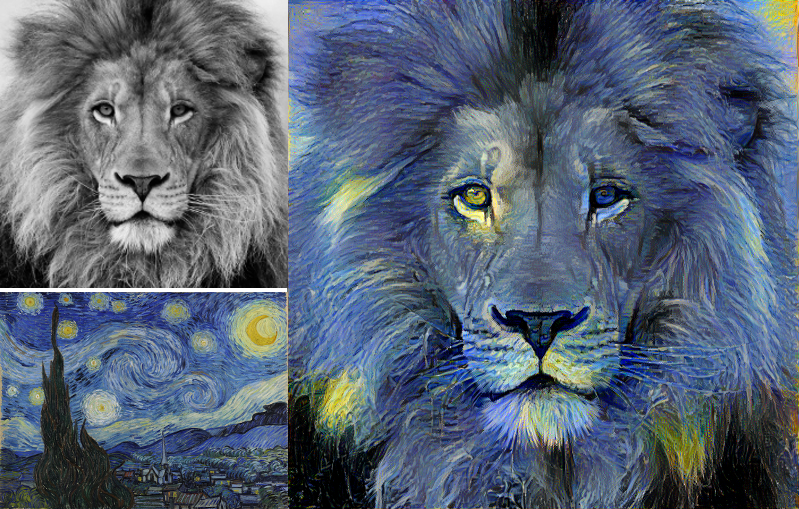
\includegraphics[width=110mm]{figures/prenos_sloga.png}
% ref: https://github.com/cysmith/neural-style-tf
\caption{Primer uporabe prenosa sloga slike z uporabo CNN}
\label{fig:prenos_sloga}
\end{figure}

V zadnjih letih je bilo precej razvoja za prenos sloga z uporabo globokih nevronskim mrež. Gatys et al. \cite{prenos_sloga} so predlagali pristop, ki uporabi inovativen pristop k zaznavi slog umetniške slike in njenega prenosa na druge slike. S pomočjo tega algoritma ohranjajo slog nanosov s čopičem, geometrijskih oblik in slikarskih struktur. Uporabljajo visoko nivojsko predstavitev lastnosti skrite plasti, ki jo dobimo s CNN. Vsebina in slog slike se podata kot dva ločena vhoda v algoritem, zato lažje dobimo model umetniškega sloga. To dosežejo z oblikovanjem optimizacijskega problema, ki se začne reševat z belim platnom. Nato po korakih išče novo podobo, ki bi sprožila podobne nevronske aktivacije kot vsebina slike in podobne korelacije lastnosti, izraženo z Gramovo matriko.

\subsection{Ohranjanje barve slike}

\begin{figure}
\centering
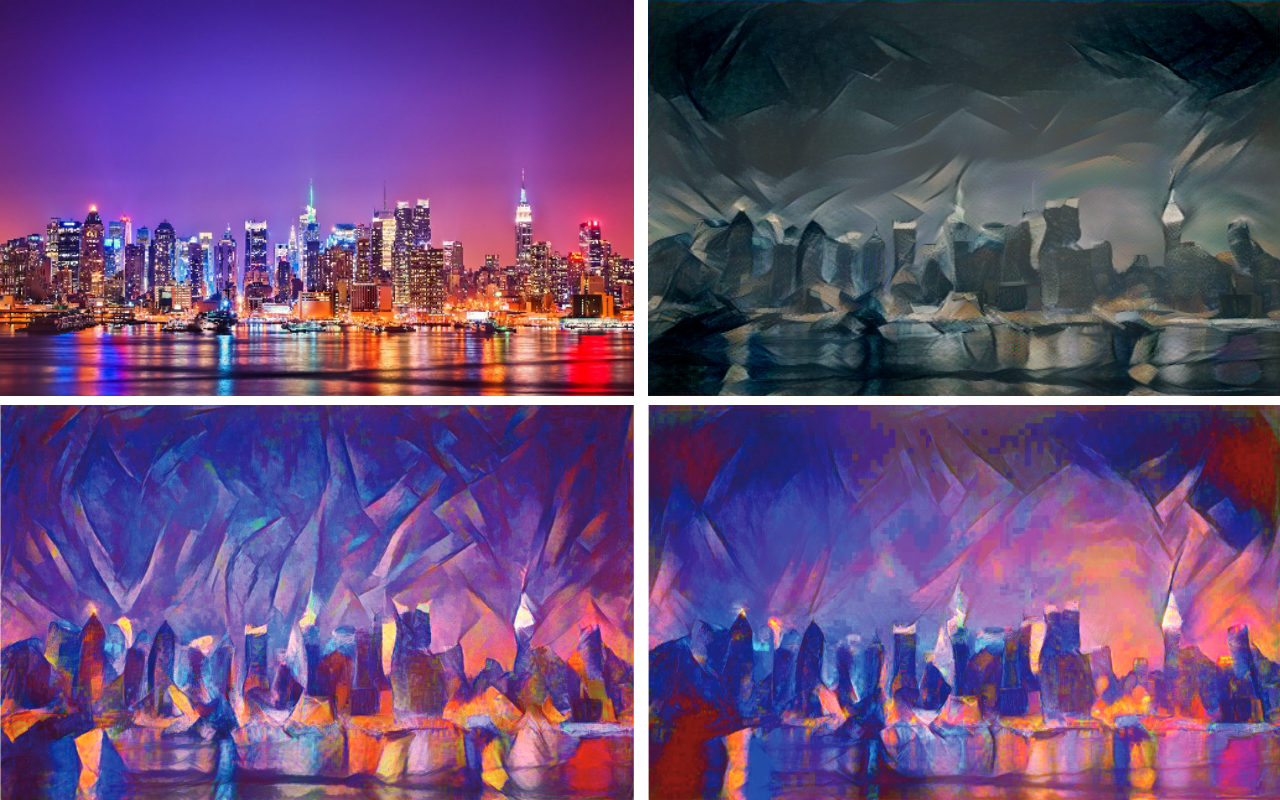
\includegraphics[width=120mm]{figures/prenos_barve.png}
% ref: https://github.com/cysmith/neural-style-tf
\caption{Primer ohranjanje barve pri prenosu sloga slike z uporabo CNN. Na spodnji levi sliki je prikazan postopek z ujemanjem barvnega histograma, na sliki desno spodaj pa prenos sloga z uporabo svetlosti}
\label{fig:prenos_barve}
\end{figure}

Z uporabo prej opisanega postopka \ref{sub:prenos_sloga} dobimo kvalitetno preslikavo slikarskega sloga, vendar hkrati izgubimo tudi barve na originalni sliki. Gatys et al. \cite{prenos_barve} so se lotili tega problema z dvema pristopoma: 

\begin{itemize}
\item \textbf{ujemanje barvnega histograma:} linearen prenos barve izbrane slike na umetniško sliko, preden jo podamo v nevronsko mrežo. Pri tem smo omejeni s kvaliteto prenosa barv, ki je težji pri bolj različnih slikah. Poleg tega se pri združevanju ohranijo vsebinske strukture slike, predvsem ostre poteze na umetniški sliki.

\item \textbf{prenos sloga z uporabo svetlosti:} iz obeh slik se prenese plast svetlosti, nad katerima se potem uporabi algoritem nevronskih mrež. Izhod potem združimo z barvo originalne slike, s čimer dobimo končno sliko. S tem se v celoti ohranijo barve, vendar se izgubi povezava med plastjo svetlosti in barve pri umetniški sliki. To se opazi predvsem pri močnih potezah čopiča, ki jim ta postopek lahko da cel spekter barv. S tem postopkom poleg tega optimiziramo tudi grajenje nevronske mreže, saj zmanjšamo nabor parametrov za eno tretjino.
\end{itemize}

%\section{Realizacija projekta}


%\subsection{Opis projektne zasnove}
\section{Implementacija}
V sklopu tega projekta smo razvili sistem, ki bo s pomočjo knjižnic, ki uporabljajo mreže CNN, obdeloval fotografije. 

Na čelnem delu (angl. \textit{frontend}) smo razvili \textit{Android} aplikacijo, ki omogoča zajem fotografije s pomočjo kamere ali izbor slike iz galerije naprave. 

%Ko bo uporabnik fotografijo zajel, jo bo aplikacija poslala na strežnik, kjer bo fotografija nadalje obdelana s pomočjo različnih zgoraj omenjenih knjižnic glede na zahteve uporabnikove. V zaledju (angl. \textit{backend}) bomo implementirali strežnik, ki bo stregel zahtevke \textit{Android} uporabnikov in koordiniral uporabo knjižnic CNN. Ko bo fotografija na strežniku dokončno obdelana, jo bo strežnik skupaj z ostalimi detekcijskimi podatki modificirano vrnil uporabniku. Rezultat uporabniške akcije bo tako strojno obdelana lastna fotografija uporabnika.

Ko uporabnik zajame fotografijo oziroma jo izbere iz galerije, aplikacija fotografijo pošlje na strežnik. Tam je fotografija nadalje obdelana s pomočjo različnih zgoraj omenjenih knjižnic mrež CNN. 

Sistem je v osnovi sestavljeni iz zalednega in čelnega dela. Zaledni del predstavljajo strežnik in sistemi za obdelavo slik z uporabo mrež CNN. Členi del predstavlja aplikacija \textit{Android}. V zaledju (angl. \textit{backend}) smo implementirali strežnik, ki bo stregel zahtevke \textit{Android} uporabnikov in koordiniral uporabo knjižnic CNN. Ko je fotografija na strežniku dokončno obdelana, jo strežnik vrne uporabniku. Rezultat uporabniške akcije je tako lastna fotografija uporabnika obdelana s pomočjo nevronskih mrež.


\subsection{Miselni vzorec ideje izvedbe projekta}

% https://app.mindmup.com/map/_free/eda28ee0130411e7a10a3343dba65313
\begin{figure}[H]
\centering
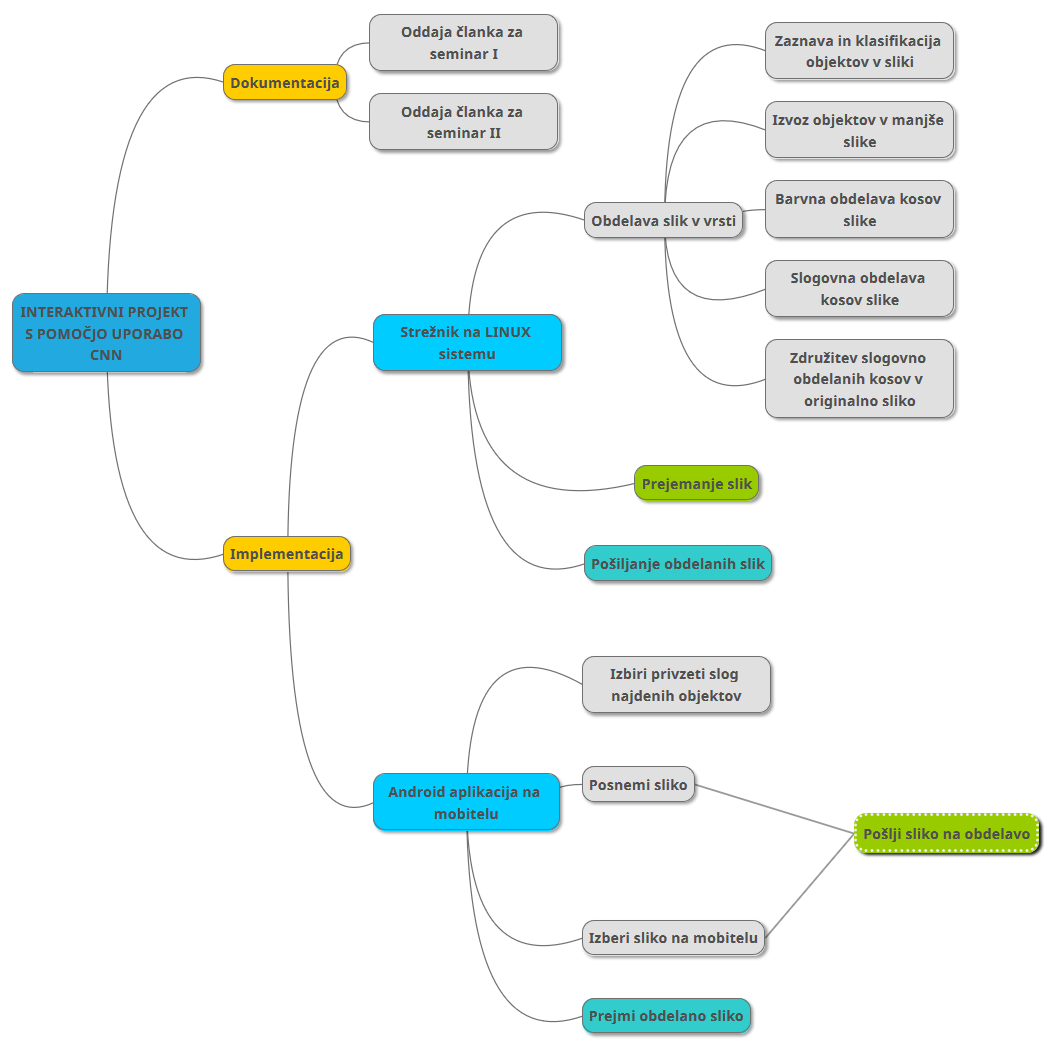
\includegraphics[width=150mm, center]{figures/mind_map.png}
% ref: https://github.com/cysmith/neural-style-tf
\caption{Miselni vzorec ideje izvedbe projekta}
\label{fig:mind_map}
\end{figure}

\pagebreak

\subsection{Načrt razvoja}

Zastavili smo naslednji načrt razvoja:
\begin{enumerate}
\item postavitev okolja in namestitev potrebnih ogrodij,
\item implementacija strežnika \textit{Butler},
\item implementacija sistema \textit{Detector},
\item integracija sistema \textit{Detector} in strežnika \textit{Butler},
\item implementacija sistema \textit{Artist},
\item integracija sistema \textit{Artist}, sistema \textit{Detector} in strežnika \textit{Butler},
\item implementacija čelne aplikacije \textit{Magician} in
\item testiranje zgornjih sistemov.
\end{enumerate}

\subsection{Sistem \textit{Butler}}
Zaledje sistema smo postavili v okolju \textit{Linux}, pri čemer smo izbrali distribucijo \textit{Ubuntu 16.04}. Strežnik smo implementirali s pomočjo ogrodja \textit{ASP.NET Core}\cite{wiki:asp_net_core}, ki je odprtokodno ogrodje namenjeno zaledni strani spletnih aplikacij. Ogrodje \textit{ASP.NET Core} deluje na različnih platformah, namenjeno je programiranju s pomočjo programskega jezika C\#. Strežnik, ki smo ga poimenovali \textit{Butler}, in odjemalec (angl. \textit{client}) bosta komunicirala preko zahtevkov protokola HTTP (angl. \textit{HyperText Transfer Protocol}). 

Ko odjemalec pošlje zahtevek HTTP POST s fotografijo, jo strežnik posreduje ustreznemu sistemu CNN, ki fotografijo glede na odjemalčev zahtevek ustrezno obdela. Ko se stiliranje fotografije zaključi, sistem CNN o uspehu procesiranja obvesti strežnik, ki obdelano fotografijo in metapodatke preko HTTP zahtevka vrne odjemalcu.

Da smo lahko strežnik objavili (angl. \textit{publish}), smo uporabili odprtokodni spletni strežnik Nginx\cite{wiki:nginx}, ki podpira objavljanje aplikacij \textit{ASP.NET Core} na platformi \textit{Linux}.

\subsection{Sistem \textit{Detector}}
Na strežniku smo poleg sistema \textit{Butler} postavili dva sistema CNN. Prvi sistem, poimenovan \textit{Detector}, uporablja jedro projekta \textit{Darknet} in je implementiran s pomočjo programskega jezika C in platforme CUDA. Glavna naloga sistema \textit{Detector} je prepoznavanje zanimivih regij oziroma objektov v sliki in predikcija kategorije zaznanega objekta. 

Komunikacijo med sistemoma \textit{Butler} in \textit{Detector} smo implementirali s pomočjo preusmerjanja standardnega izhoda in vhoda. Ko se sistem Butler postavi, se obenem v ozadju inicializira storitev \textit{DetectorService}, ki zažene sistem \textit{Detector}. Sistem \textit{Detector} ob zagonu naloži uteži v grafični pomnilnik in nato v neskončni zanki čaka na naloge sistema \textit{Butler}. Zgoraj omenjena storitev \textit{DetectorService}, ki skrbi za delegacijo nalog sistemu \textit{Detector}, določa vrstni red operacij s pomočjo podatkovne strukture vrsta (angl. \textit{queue}) po sistemu prvi noter, prvi ven (angl. \textit{First In, First Out} - FIFO). S tem smo programsko zagotovili, da lahko sistem \textit{Detector} naenkrat obdeluje največ eno fotografijo.

V primeru, ko sistem \textit{Detector} v fotografiji zazna več regij, pri združevanju začnemo združevati z regijo pri kateri je bilo zaupanje napovedi tipa zaznanega objekta najmanjše in postopoma nadaljujemo do regij, pri katerih je bilo zaupanje večje. Tako na končni sliki vedno prevlada stil objekta z največjim zaupanjem.

Na sliki \ref{fig:input_detector} je prikazana zaznava regij v sistemu \textit{Detector} in na sliki \ref{fig:detector} izrez zaznanih regij.

\begin{figure}[H]
\centering
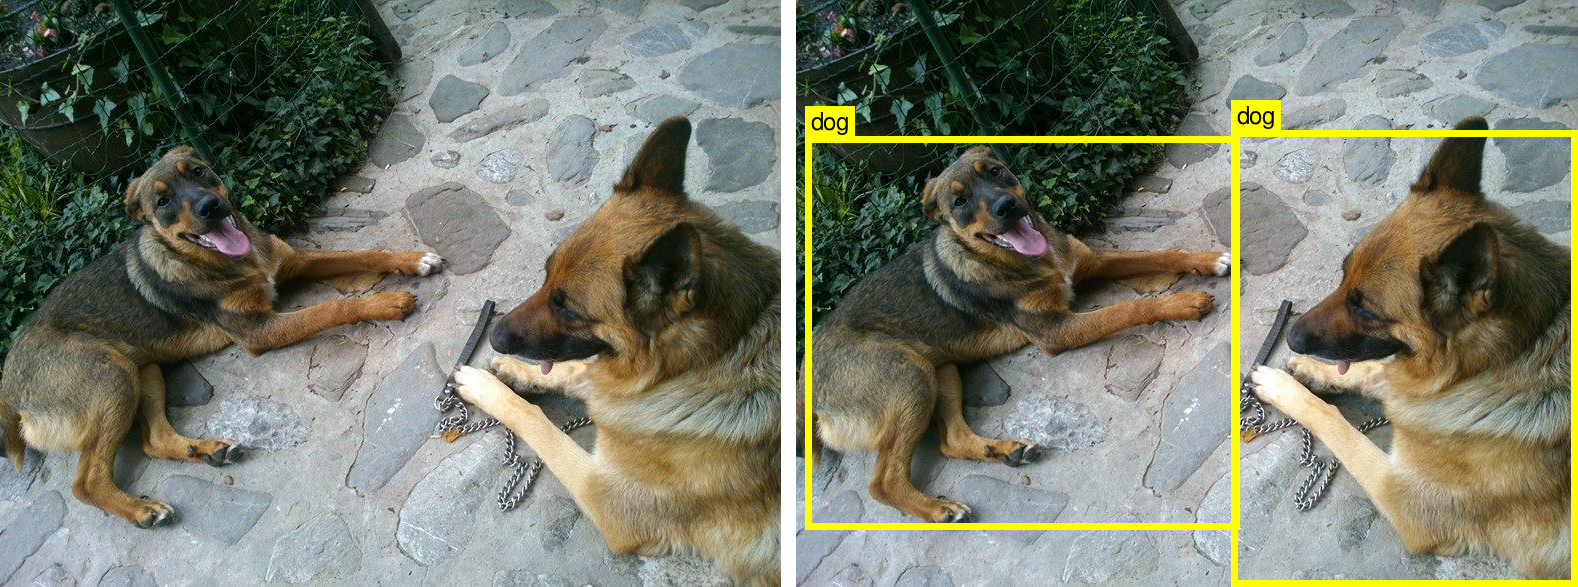
\includegraphics[width=\textwidth, center]{figures/neural_example/input_detector.png}
\caption{Zaznava regij v sistemu \textit{Detector} iz vhodne slike}
\label{fig:input_detector}
\end{figure}

\begin{figure}[H]
\centering
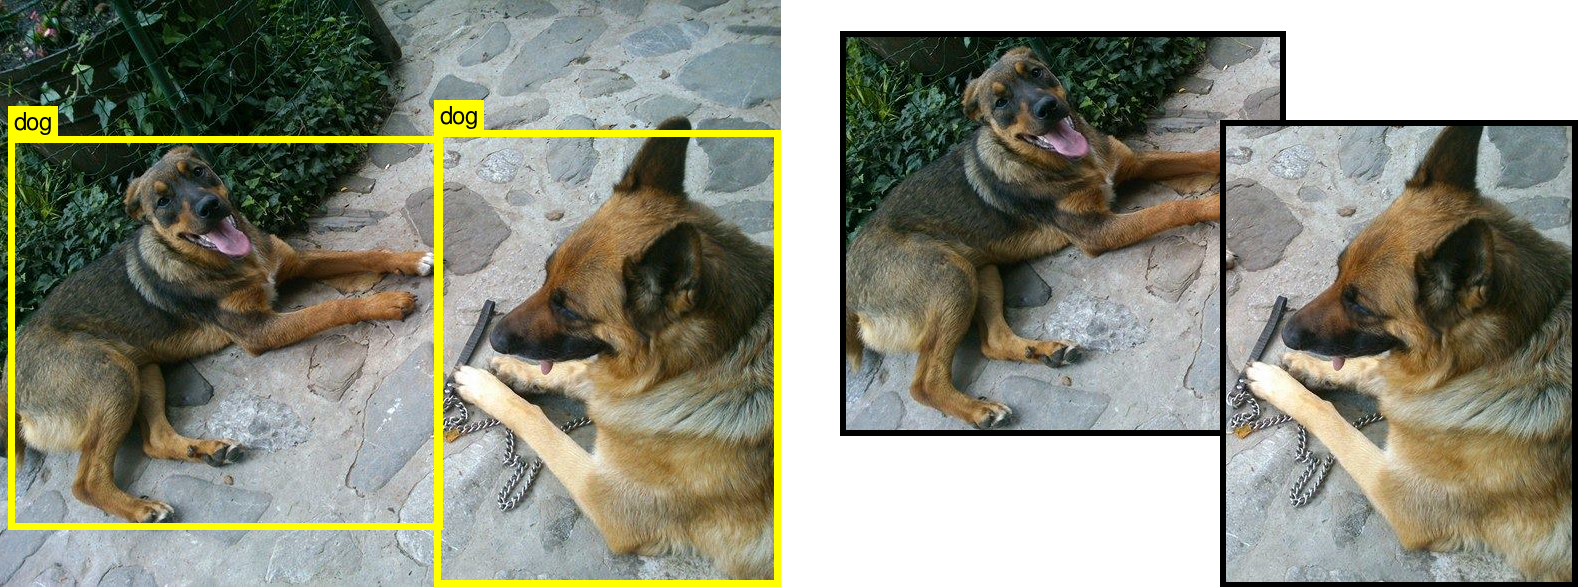
\includegraphics[width=\textwidth, center]{figures/neural_example/detector.png}
\caption{Izrez zaznanih regij v sistemu \textit{Detector}}
\label{fig:detector}
\end{figure}

\subsection{Sistem \textit{Artist}}
%EDITED
Sistem \textit{Artist} temelji na implementaciji knjižnice TensorFlow v jeziku Python za treniranje hitre nevronske mreže za prenos stila \cite{neural-style-fast}. Uporabljene so podobne transformacije mreže kot pri \cite{neural-style-johnson}, ki je sicer implementiran s knjižnico Torch. Normalizacija skupine vhodnih podatkov je narejena z Ulyanovo instanco. Za večjo zmogljivost je bila celotna knjižnica Tensorflow prevedena v binarno kodo na strežniku. Poleg tega smo omogočili še grafično pospeševanje s knjižnicama CUDA in CUDNN, ki ju nudi Nvidia, vendar zahtevata precej zmogljivo grafično kartico z vsaj 4GB grafičnega pomnilnika.

Za apliciranje stilov na zaznane regije sistem uporablja uteži, ki opisujejo potrebne transformacije za pretvorbo. Da stiliranje regij poteka dovolj hitro, sistem uporablja uteži, ki so naučene samo enega specifičnega stila. S sistemom se je sicer možno z predpripravljenimi podatki \cite{vgg-19} naučiti novih transformacij s poljubno sliko, vendar ta proces vzame od 4 do 6 ur na \textit{ Maxwell Titan X} grafični kartici.

Podobno kot pri sistemu \textit{Detector}, sistem \textit{Butler} delegira naloge sistemu \textit{Artist} s pomočjo vrste (angl. \textit{queue}). Sistem \textit{Artist} začne z apliciranjem sloga, ko mu sistem \textit{Butler} posreduje informacijo, da je nov nabor zaznanih regij v čakalni vrsti pripravljen na obdelavo. Te regije ustvari sistem \textit{Detector} po opravljeni detekciji artefaktov, kjer iz originalne slike izreže zanimive dele in jih posreduje v prej omenjeno čakalno vrsto. Sistemu \textit{Artist} sistem \textit{Butler} posreduje pot do direktorija, ki vsebuje zaznane regije, in pot do uteži želenega stila.

Obdelava posamezne regije se začne z nalaganjem nevronske mreže izbranega sloga v grafični pomnilnik, kjer ostane do konca procesa. Operacija stiliranja tipično traja okoli 5 sekund na grafični kartici \textit{GTX 960M}, časovna zahtevnost je odvisna predvsem od velikosti slike. Poleg tega smo lahko hkrati še omejeni glede maksimalne resolucije, saj nam lahko pri manjši kapaciteti grafične kartice zmanjka grafičnega pomnilnika. Ko je delo zaključeno, se vse slike shranijo na svoje mesto v podatkovni bazi.

Ko je stiliranje zaključeno, sistem \textit{Artist} o tem obvesti sistem \textit{Butler}. Ta regije nato prilepi nazaj na njihovo mesto v originalni sliki in s pravokotniki označi zaznane objekte, ki se naj bi tam nahajali. To združeno sliko sistem \textit{Butler} shrani v podatkovno bazo, s čimer se zaključi obdelovanje slike in obvesti sistem \textit{Magician}, da lahko uporabniku vrne sliko.

Na sliki \ref{fig:detector_artist} je prikazano apliciranje sloga na izrezane zaznane regije v sistemu \textit{Artist} in na sliki \ref{fig:merged} končno združevanje originalne fotografije in zaznanih regij v sistemu \textit{Butler}.

\begin{figure}[H]
\centering
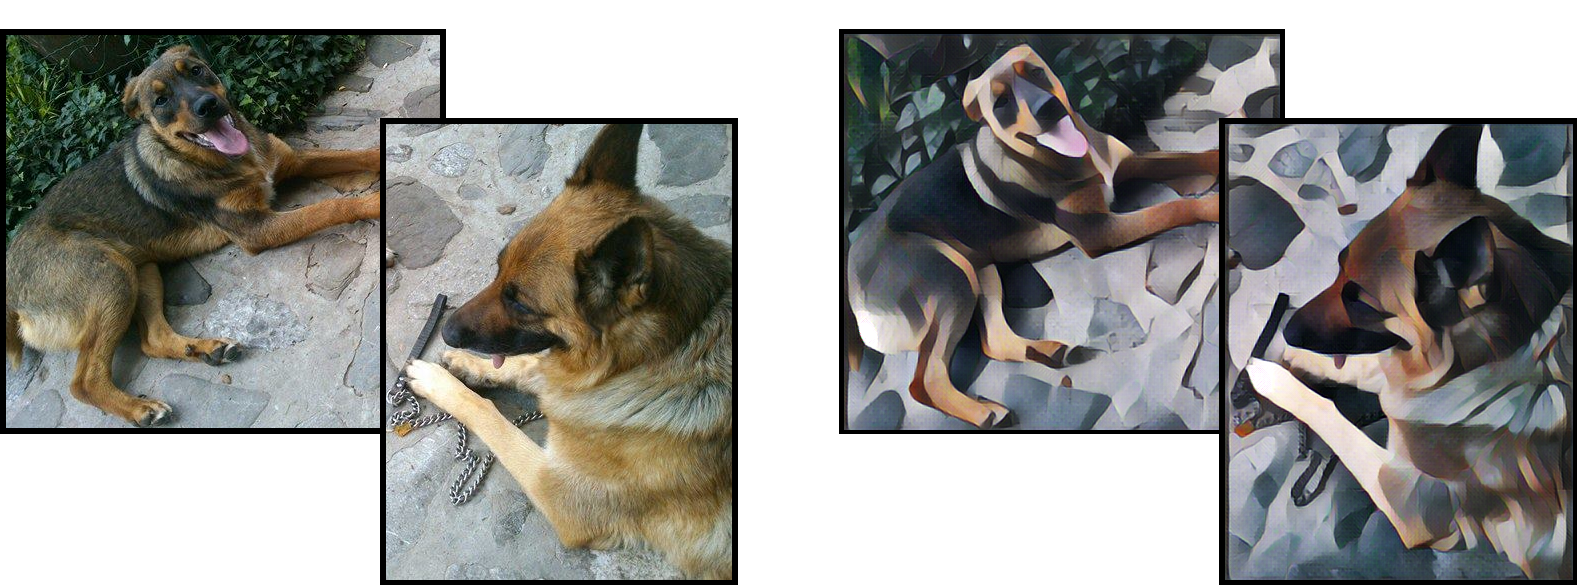
\includegraphics[width=\textwidth, center]{figures/neural_example/detector_artist.png}
\caption{Apliciranje sloga na izrezane zaznane regije v sistemu \textit{Artist}}
\label{fig:detector_artist}
\end{figure}

\begin{figure}[H]
\centering
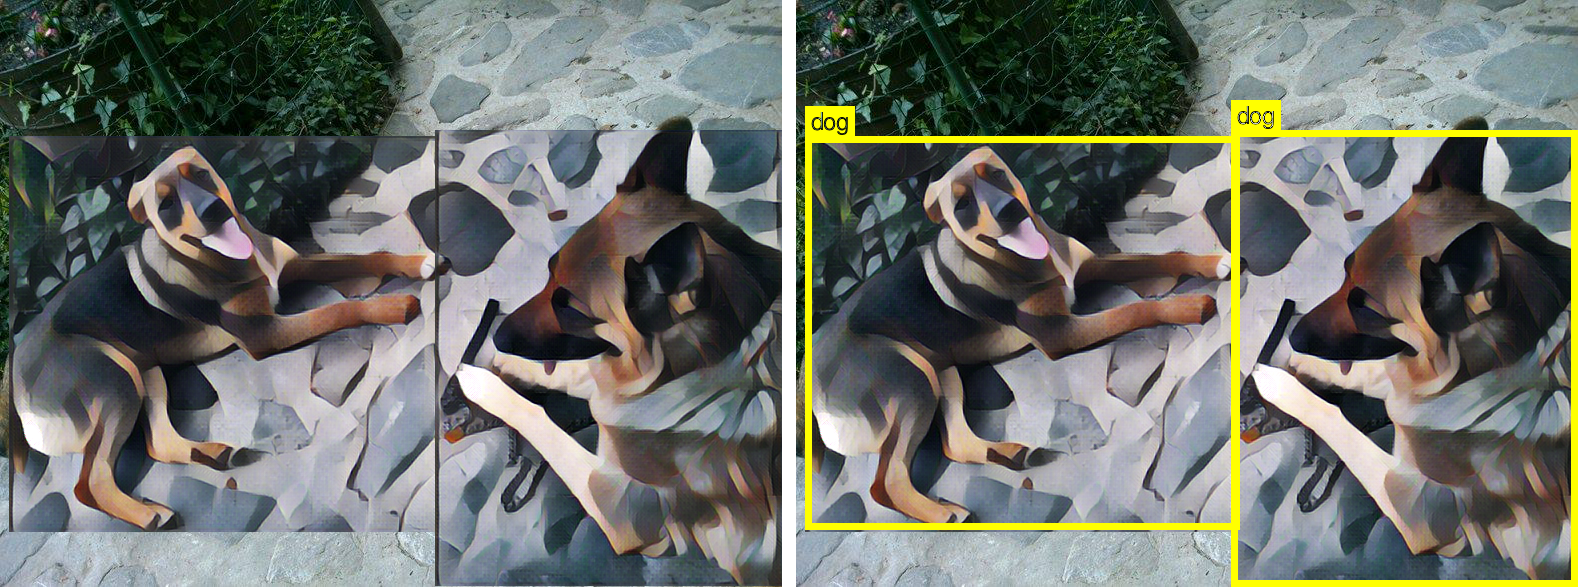
\includegraphics[width=\textwidth, center]{figures/neural_example/merged.png}
\caption{Končno združevanje originalne fotografije in zaznanih regij v sistemu \textit{Butler}}
\label{fig:merged}
\end{figure}

\subsection{Podatkovna baza}
Podatkovno bazo smo implementirali s pomočjo shranjevanja fotografij na disk. Ob vsakem prejetem zahtevku HTTP POST ustvarimo unikatno identifikacijsko številko zahtevka, ki jo določimo s pomočjo časovnega žiga. Nato v mapi, ki predstavlja podatkovno bazo, ustvarimo podmapo, katere ime ustreza zgornji identifikacijski številki. Takoj po prejemu zahtevka sistem \textit{Butler} v mapi shrani originalno fotografijo. Ko kasneje sistem \textit{Detector} zaključi z detekcijo, v mapo zahtevka shrani fotografijo z zaznanimi regijami. Prav tako v podmapi \textit{detector} shrani slike, ki predstavljajo posamezne zaznane regije, izrezane iz originalne fotografije.

Nato sistem \textit{Artist} izrezane fotografije iz podmape \textit{detector} eno za drugo obdela, tako da nanje aplicira željeni slog in jih shrani v novo podmapo \textit{artist}.

Na koncu sistem \textit{Butler} iz originalne fotografije in posameznih fotografij iz podmape \textit{artist} sestavi končno fotografijo, ki predstavlja rezultat obdelave. 

V mapi vsakega zahtevka poleg fotografij hranimo tudi objekt \textit{ImageTask}, ki vsebuje metapodatke o posameznem zahtevku. Zgornji objekt je shranjen v odprtokodnem formatu JSON (angl. \textit{JavaScript Object Notation}).

\subsection{Sistem \textit{Magician}}
Uporabnik lahko izkoristi funkcionalnosti implementiranih algoritmov s pomočjo namenske aplikacije \textit{Android}, poimenovano \textit{Magician}. Razvita je z razvojnim okoljem \textit{Android Studio}, in podpira večino naprav, ki uporabljajo ta operacijski sistem. 

Ob zagonu aplikacije lahko uprabnik s pomočjo knjižnice za komunikacijo s kamero \cite{camera-view} posname sliko ali pa jo naloži iz galerije naprave. Izbrana slika se nato pošlje na strežnik preko HTTP POST zahtevka. Nato aplikacija \textit{Magician} vsako sekundo pošlje zahtevek HTTP, s katerim jo sistem \textit{Butler} obvešča o trenutnem napredku obdelave. Ko je slika obdelana, jo aplikacija pridobi s strežnika s pomočjo zahtevka HTTP GET in jo prikaže uporabniku. Rezultat operacije je tako obdelana slika, na kateri so razvidne zaznane regije in nanje apliciran slog. Na koncu lahko uprabnik sliko shrani v galerijo naprave.

\subsection{Shema sistema}
Na sliki \ref{fig:system_scheme} je vidna shema celotnega sistema in pot enega primera zahtevka uporabnika.

\begin{figure}[H]
\centering
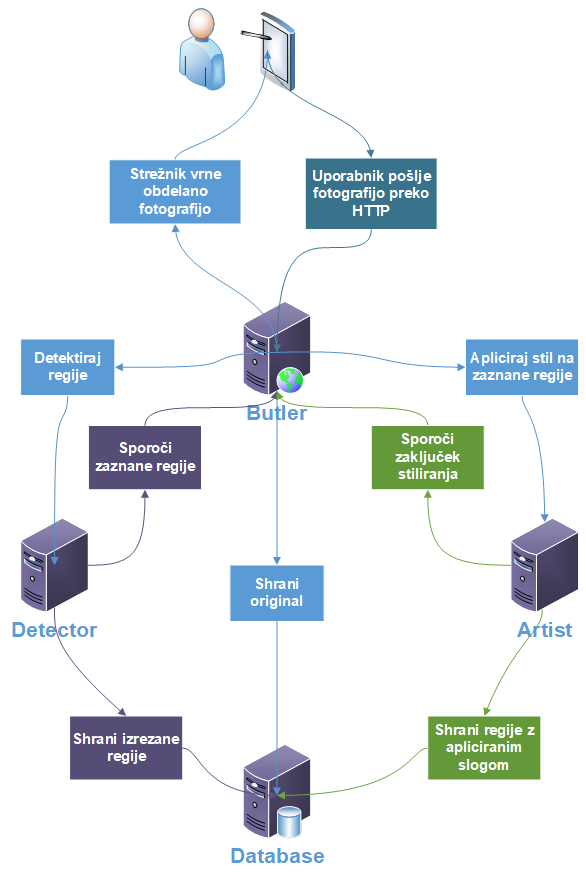
\includegraphics[width=135mm, center]{figures/vzorec.png}
% ref: https://github.com/cysmith/neural-style-tf
\caption{Shema celotnega sistema}
\label{fig:system_scheme}
\end{figure}

\section{Zaključek in nadaljnje delo}
Implementacija strežnika in vseh ostalih sistemov, ki jih uporablja, je precej dobro zastavljena in verjetno ne potrebuje večjih nadgradenj. Ker se pri obdelavi slik uporablja čakalna vrsta, lahko naenkrat strežemo več uporabnikov brez zapletov. Večja omejitev je le pri zmogljivosti strojne opreme, kjer bi bila za hitrejše zaznavanje regij na sliki in njihovo stiliranje zaželjena močnejša grafična kartica. Poleg tega je z učenjem mogoče razširiti paleto stilov pri sistemu \textit{Artist}, vendar je potrebna večurna obdelava s pomočjo grafične kartice. 

S sistemom \textit{Artist} je mogoče stilirati tudi videe, tako da bi lahko dodali to funkcionalnost v sistem \textit{Butler}.

Na Android aplikaciji \textit{Magician} bi lahko opravili še veliko dela, zato da bi uporabniku omogočili več izbire pri manipulaciji izgleda končne slike. Možne nadgradnje so: 
\begin{itemize}
\item izbira stila za vsako najdeno regijo posebej
\item možnost odstranitve pravokotnikov in napisov, ki označujejo regije
\item spreminjanje meje občutljivosti za zaznavanje regij
\item stiliranje celotne slike
\end{itemize}

\bibliographystyle{plain}
\bibliography{literatura}

\end{document}
